\documentclass{article}
\usepackage[utf8]{inputenc}
\usepackage[english]{babel}
\usepackage{abstract}
\usepackage{tabularx}
\usepackage{graphicx}
\usepackage[round]{natbib}
\usepackage{url}
\usepackage{hyperref}
\hypersetup{
    colorlinks=false, %set true if you want colored links
    linktoc=all,     %set to all if you want both sections and subsections linked,
}

\usepackage[style=numeric,backend=bibtex]{}

\title{A Technical And Ethical Analysis Of `Automatic and Predictive Traffic Light Systems for Public Roads' In The Context Of The European AI Act}
\date{December 4, 2022}
\author{
        \textit{Aravindh Ramasamy}\\
        \textit{Benedikt Schwankner}\\
        \textit{Uppili Srinivasan}\\
        \textit{David-Peregrin Hain}\\
        \textit{Till-Ole Lohse}
  %% \and \ldots
}

\begin{document}
  \maketitle

  \begin{abstract}
    This is a paper for educational purposed written by five students of \emph{TUM for the The EU’s Draft AI Act: From framework to practical application} Seminar in the WS 22/23. In this paper we wrote an introduction to the EU's Draft AI Act and the Fraunhofer’s \emph{Automatic and Pre-dictive Traffic Light Systems for Public Roads}. Following this we applied the Articles of the AIA to the AI system of Fraunhofer and wrote a technical documentation with the information we got from them about the model as required by the AIA. The paper is closed by a ethical analysis of any dangers this system poses.
  \end{abstract}
  \newpage
  
  \tableofcontents

  \section{Introduction to EU's Artificial Intelligence Act: The European Approach to AI}
    In order to understand the research project and the associated system for automatic and predictive traffic guidance of the Fraunhofer Institute in detail, a general look at the European Commission's draft of the EU Artificial Intelligence Act will be discussed beforehand.\\
    On April 21, 2021, the European Commission presented its proposal for a regulation that would provide harmonized rules for the use and management of artificial intelligence (AI) in the EU - in short, the AI Act. The draft regulation aims to standardize the approach to AI and, in particular, to align it with the EU's high standards of trustworthy AI. [\citet{kop2021eu}]. The proposed Regulation sets out fundamental rules for the development, commercialization, and utilization of AI-driven products, services, and systems in the territory of the EU, applicable to all industries. For the implementation of this, a system based on four risk categories has been developed, which sets different compliance rules at the respective risk levels. [\citet{ebers2021standardizing}] The AI Act suggests categorizing AI systems into four levels of risk based on threats to health, safety, and constitutional rights, 1. unacceptable, 2. high, 3. limited, and 4. minimal.  [\citet{lutge2022risk}] This risk-based approach based on the criticality pyramid (see below) is combined with a sophisticated, multi-level regulatory enforcement mechanism. As a result, stricter rules apply as the risk increases. AI systems that pose unacceptable risk are prohibited, high-risk AI systems face a long list of pre-market and post-market requirements. Limited-risk AI systems are governed by transparency obligations, and minimal- to no-risk AI systems can be used liberally.\\

    \begin{figure}[h]
        \centering
        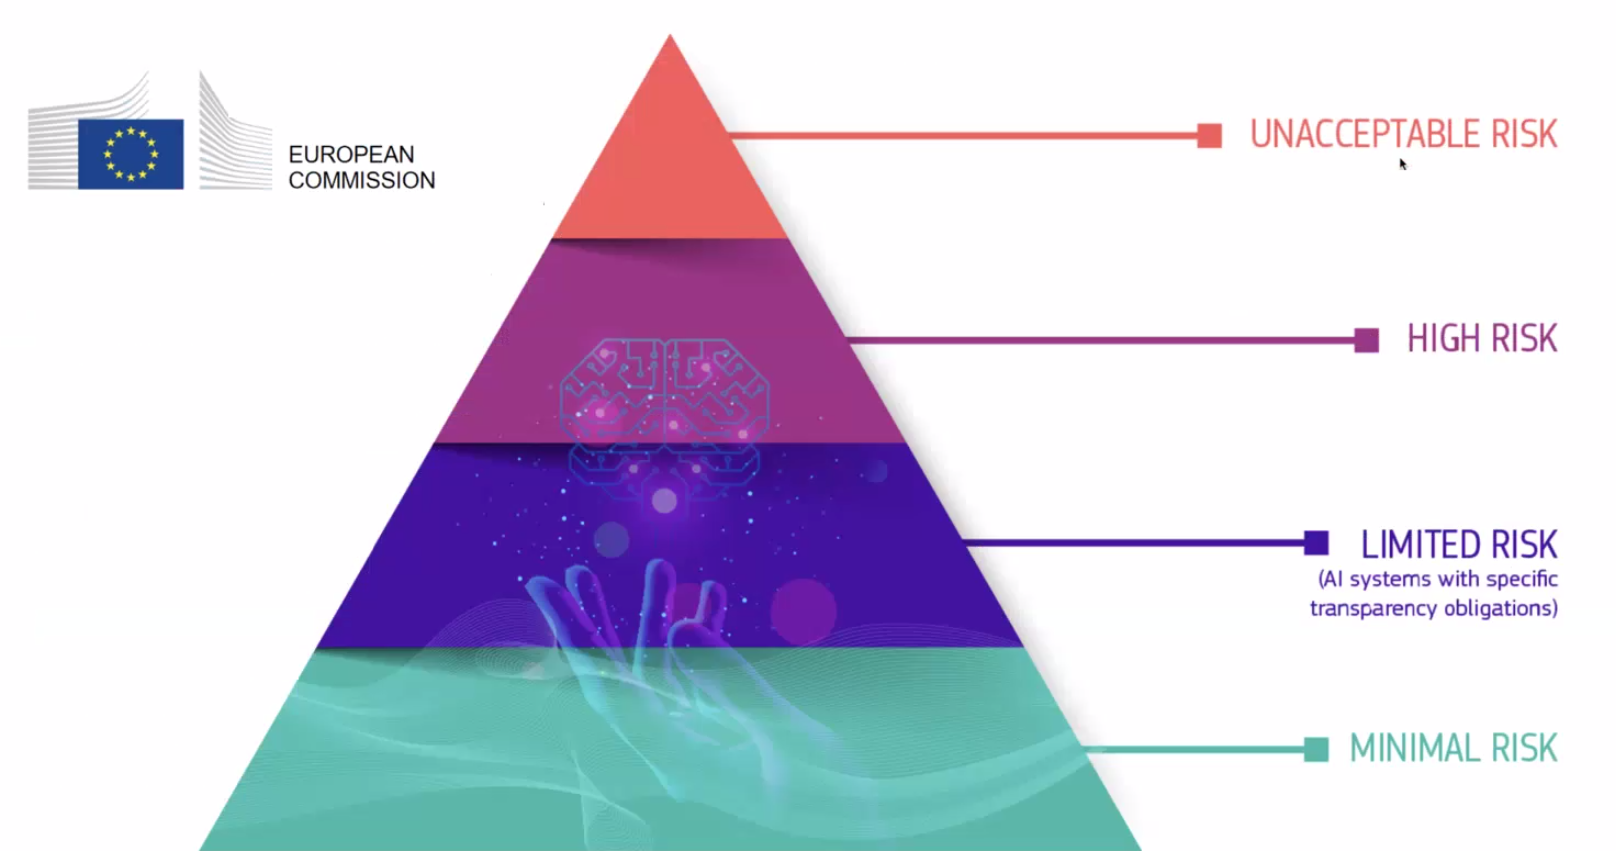
\includegraphics[width=0.8\textwidth]{paper-template/figs/risk_levels.png}
        \caption{Risk-based approach - Pyramid of risks (EU Commission, 2021) }
        \label{fig:my_label}
    \end{figure}
    Under the proposed Article 10 of the EU AI Act, an intent is not only to regulate the placing on the market of AI systems, but also to regulate the scope of training, testing, and validation data sets for AI systems that utilize machine learning.\\
    Fines for non-compliance can be as high as 6\% of global turnover for companies. The European Commission is trying to strike a balance with AI Act. On the one hand, it wants to prevent regulations from stifling innovation, and on the other hand, it wants to hinder the creation of an unrestrained AI ecosystem in Europe (also by introducing legal sandboxes that give AI developers room to maneuver). [\citet{fink2021eu}] The EU AI Act can be understood as groundbreaking in terms of the whole ecosystem. [\citet{kop2021eu}]\newline\newline
    The traffic light and traffic management system, which is currently being developed by the Fraunhofer Institute's branch for industrial automation, can be classified as a high-risk AI system (for a more detailed explanation, see below). Accordingly, the regulatory framework and the classification of systems as high-risk will be analyzed in more detail subsequently.
    Title III (Article 6) of the proposed AI Act provides a definition of what is to be classified as a high-risk AI system. It refers to systems that would have a negative impact on the safety of people or their fundamental rights. The draft law further distinguishes between two categories of high-risk AI systems.  [\citet{madiega2021artificial}] Firstly, systems with a high risk due to their use as safety components or any products that fall under the harmonization regulations of the European Union for safety and health protection. This is, for example, the use of AI in the field of toys, aviation, medical devices, passenger elevators or similar. [\citet{ebers2021standardizing}] Secondly, as described in Article 7, high-risk AI systems which are deployed one of the following: "Biometric identification and categorization of natural persons; management and operation of critical infrastructure; education and training; employment, workforce management, and access to self-employment; access to and use of essential private and government services and benefits; law enforcement; migration, asylum, and border control management; administration of justice and democratic processes." (Excerpt from Annex III of the Proposal for the EU AI Act).\\ \newline
    All of these systems that fall into the above categorization as high-risk AI systems thus have the following regulations imposed on them: \textbf{Require up-front conformity assessment:} The development of a high-risk system should ideally be done using "internal ex-ante AI Impact Assessments and Codes of Conduct overseen by inclusive, multidisciplinary teams”. [\citet{kop2021eu}]
    \textbf{Registration in the special EU database:} Providers of high-risk AI systems will be obliged to register their systems in an EU-wide database managed by the EU Commission before they launch their product on the market. \textbf{Declaration of Conformity (throughout the entire lifecycle):} The system must be approved by conformity assessment and must satisfy the corresponding requirements specified in the EU AI Act throughout its entire life cycle. Also, the Hi-Risk AI system must bear the CE marking (Conformité Européenne)\newline In addition, high-risk systems must meet other additional requirements. Specifically, they must meet requirements for "risk management, testing, technical robustness, data protection and management, transparency, human oversight, and cybersecurity" [\citet{madiega2021artificial}]as set forth in Articles 8 to 15 of the proposed EU AI Act. Not only providers, but also importers, distributors and users of AI systems must comply with these requirements. Providers with their registered office outside the EU are obliged to appoint an authorized representative within the EU who ensures conformity assessment and monitors compliance with the above-mentioned requirements and, if necessary, initiates countermeasures in the event of violations.
\newline\newline
\section*{Introduction to Fraunhofer's Automatic and Predictive Traffic Light Systems for Public Roads}
  After a detailed analysis of the EU AI Act in general and high-risk systems in particular, this paper will next analyze a system that falls into the above-mentioned category and is thus interesting for the analysis of the requirements for the system design and also for the technical implementations as well as an assessment and discussion of the risks that such a system entails.\newline
The Fraunhofer Institute, based in Munich, has been researching the use of various technical innovations in road traffic for some time in order to optimize the flow of traffic, especially in cities. A research group from the Fraunhofer Institute for Optronics, System Technologies, and Image Exploitation IOSB has recently been conducting more extensive research into the use of sensor technology around intersections, combined with the use of self-learning algorithms, in order to optimize traffic flows and achieve shorter waiting times for all road users, but above all to create improved safety for pedestrians. The research team is relying on a combination of innovative sensor technology and the use of artificial intelligence to enable "intelligent, predictive light switching." [\citet{optimized_traffic_flows_and_improved_pedestrian_safety_2022}] Presently, traffic light control in Germany is based on time-controlled and rule-based algorithms combined with the use of induction loops installed on the road surface. However, this approach only conveys a rough impression of the actual traffic situation [\citet{bmdv_2022}] and, moreover, is suitable for the constantly growing traffic volume (especially in the cities) to a limited extent only. [\citet{publisher_2022}]\newline Instead of conventional sensors, the researchers at Fraunhofer IOSB-INA employ high-resolution cameras and radar sensors to capture the actual traffic situation more accurately and are thus able to determine the exact number of waiting vehicles at an intersection in real-time and also to record and track the average speed of the cars and the waiting times of the respective vehicles.  [\citet{optimized_traffic_flows_and_improved_pedestrian_safety_2022}] The data collection serves as a foundation and input parameter for artificial intelligence, which utilizing deep reinforcement learning algorithms is able to calculate the optimal switching behavior for the traffic lights and thus create the ideal phase sequence in order to shorten the waiting times at the intersection, reduce travel times, and thus reduce the noise and CO2 pollution caused by the traffic jam. [\citet{fraunhofertrustworthy}] \newline The computational resources for the AI algorithms are provided by edge computers in the control box directly at the intersection. Looking to the future, the researchers hope for another positive advantage: the system will not only be used at individual intersections but a network of neighboring traffic lights that form a larger network can be formed with it, thus optimizing and directing the flow of traffic in real-time across larger regions. [\citet{bundesministerium_für_wirtschaft_und_klimaschutz_2022}]Initial tests, which are being conducted at an intersection in Lemgo, Germany, show that the system can generate a 10-15\% improvement in traffic flow.  [\citet{optimized_traffic_flows_and_improved_pedestrian_safety_2022}]\newline
 \begin{figure}[h]
        \centering
        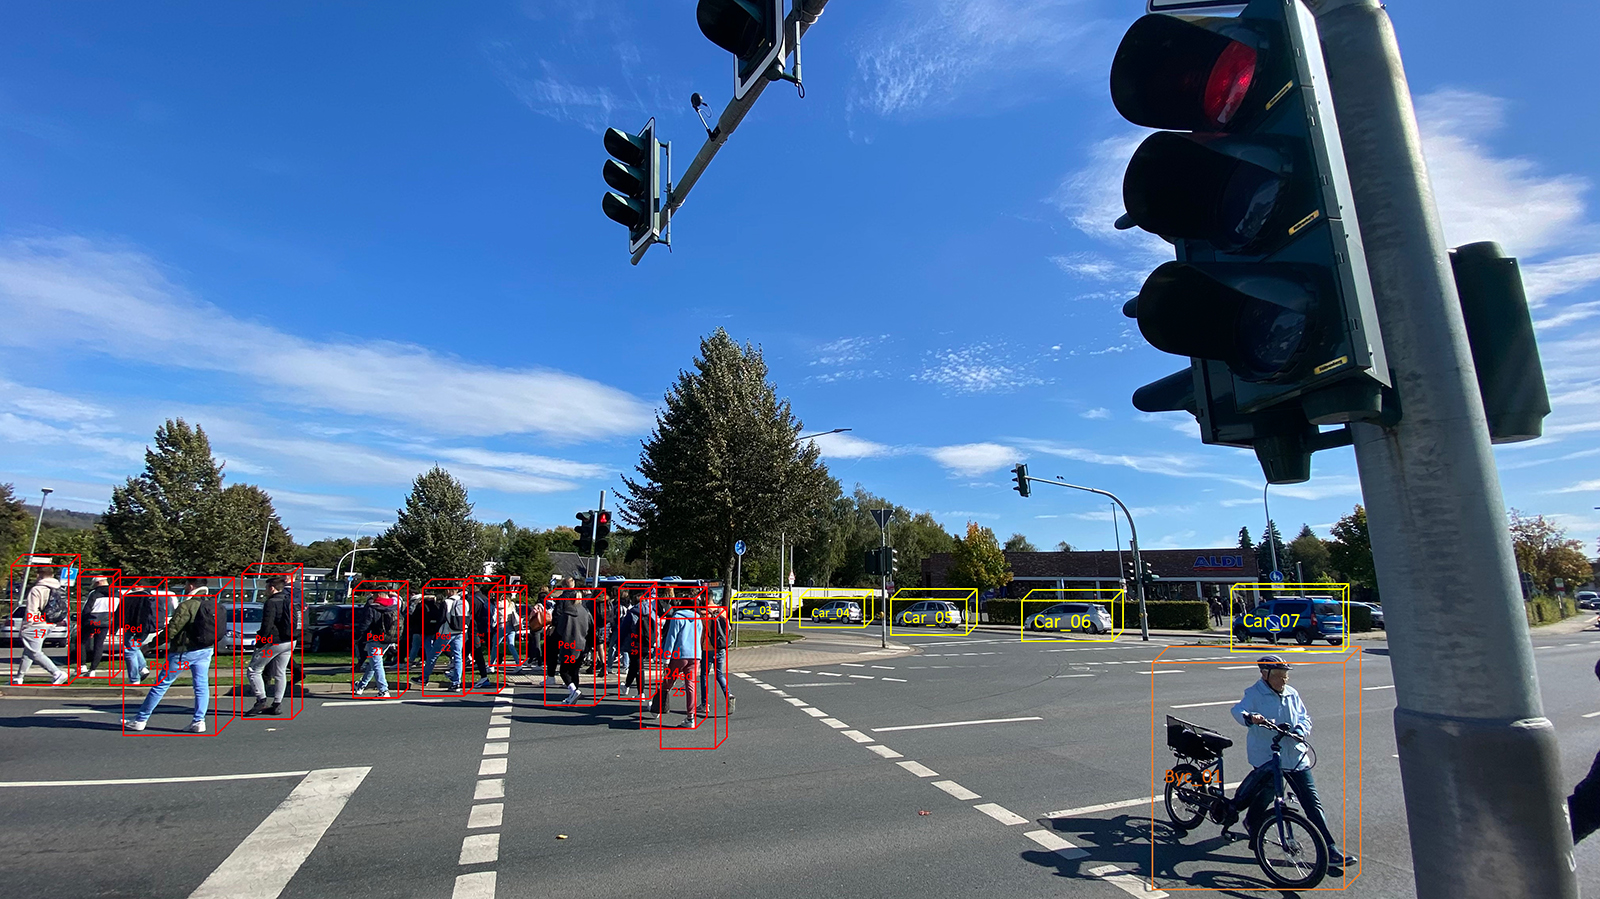
\includegraphics[width=0.8\textwidth]{paper-template/figs/traffic_lights1.jpg}
        \caption{People are detected and tracked using LiDAR sensor data and AI.}
        \label{fig:my_label}
    \end{figure}\newline
In addition to improving traffic flow, the AI-based system also aims to develop a new approach to demand-based control for pedestrian signals.  [\citet{optimized_traffic_flows_and_improved_pedestrian_safety_2022}] This is especially beneficial for vulnerable groups of people (elderly or people with disabilities). Reduce waiting times but above all increase safety at crosswalks (for example by adjusting crossing times if a person has not quite crossed the road in the time originally planned). The current solutions at traffic lights (predominantly simple buttons) are not able to meet the special needs of these groups of people. High-resolution LiDAR sensors in combination with AI can automatically adjust crossing times to the needs of pedestrians and, if necessary, extend or even shorten them to improve traffic flow at the same time. [\citet{publisher_2022}]
As a result, the research group from the Fraunhofer Institute is relying on state-of-the-art AI technology and hopes to achieve significant improvements in terms of waiting times and safety for both motorists and pedestrians with comprehensive coverage in the road network. [\citet{optimized_traffic_flows_and_improved_pedestrian_safety_2022}] The research area is divided into the two research projects KI4LSA and KI4PED, which focus on motor vehicle traffic and pedestrian traffic, respectively.\newpage
 \begin{figure}[h]
        \centering
        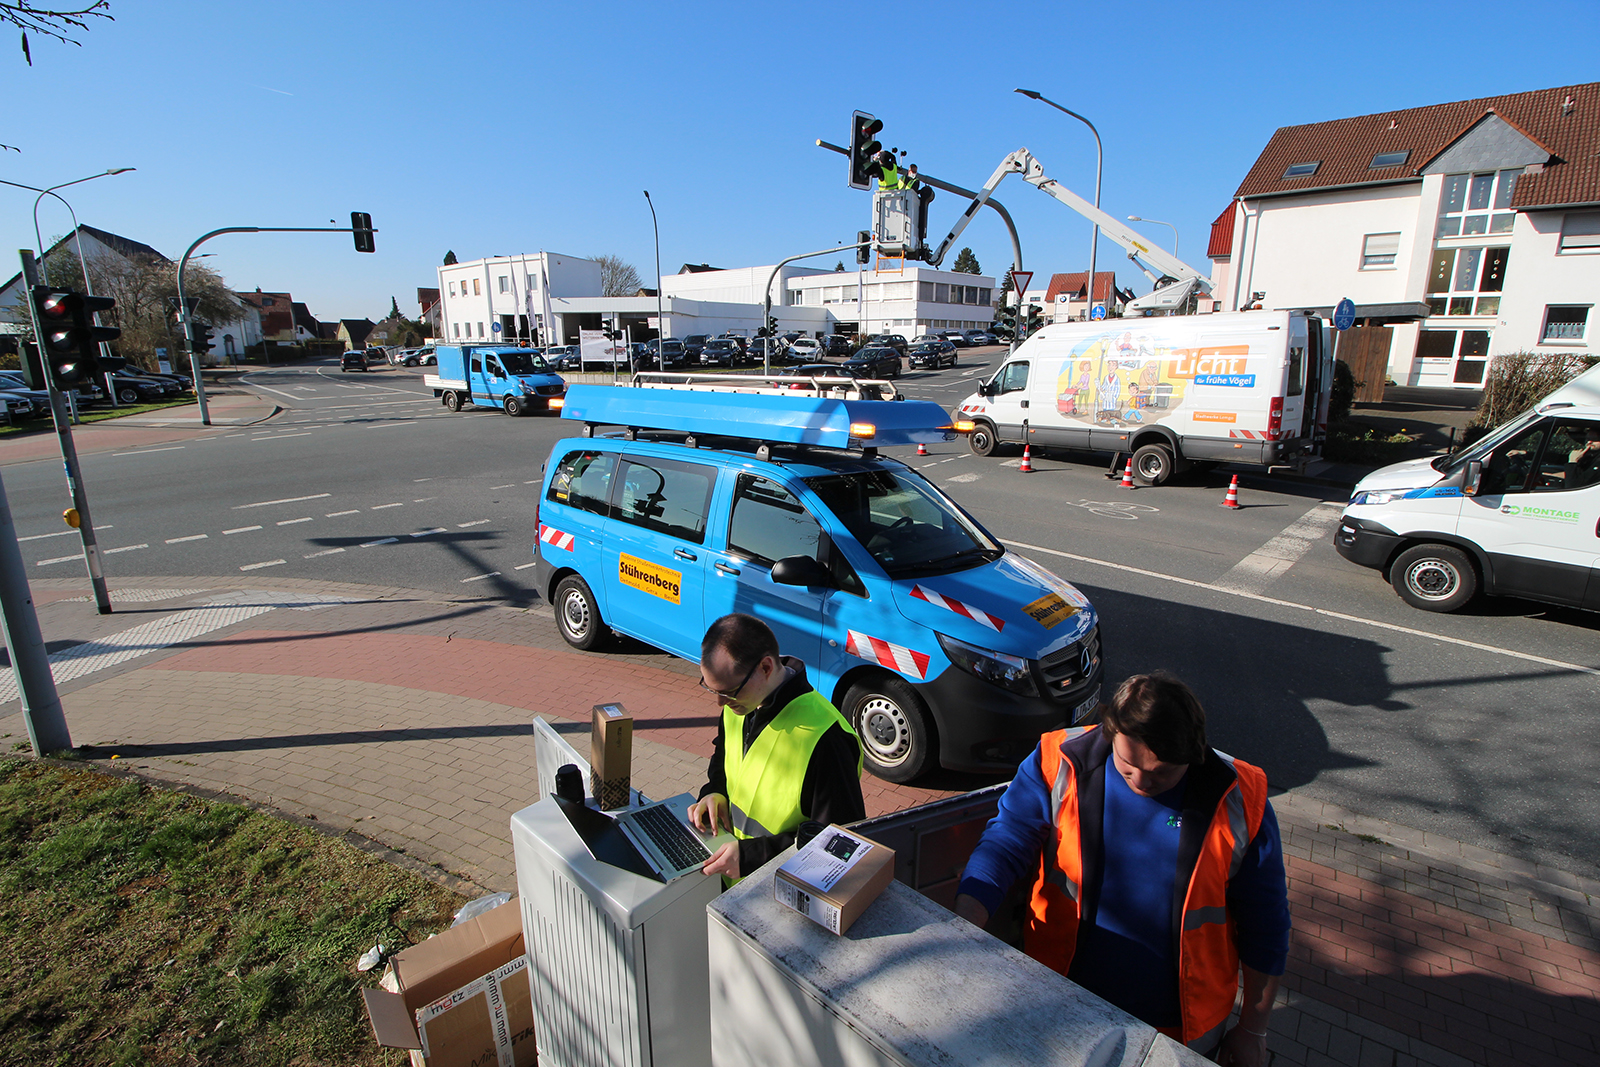
\includegraphics[width=0.8\textwidth]{paper-template/figs/traffic_light2.jpg}
        \caption{Highresolution cameras and radar sensors gather detailed traffic information.}
        \label{fig:my_label}
    \end{figure}
 \textbf{Why Fraunhofer's traffic light system should be classified as a high-risk AI tool}\newline In the previous paragraphs, a general analysis of high-risk systems, including the definition and an explanation of when an AI system is considered a high-risk AI system, has already been presented. The question, which remains unanswered so far, is whether the Fraunhofer Institute's traffic light system that has just been explained falls into the categorization of a high-risk AI System as it is lied down in the proposal of the EU AI Act.\newline
As stated in Article 6 f of the European Commission's proposal for the EU AI Act, any system is to be classified as high-risk if it is included in the list of Annex III. This includes all systems that are used in the management or operation of critical infrastructure. [\citet{madiega2021artificial}]  Use in critical infrastructure here includes, above all, all AI systems that are to be used as safety components for the management and operation of road traffic as well as water, gas, heat, and electricity supplies. \newline
Since Fraunhofer's Traffic Light System is evidently an operation within road traffic, Article 6 f necessarily applies - especially since it is clearly also intended to be used on public roads. Thus, the Traffic Light Systems might clearly be considered a high-risk AI system. 
However, the classification seems to be trivial only at first glance, since currently the technical implementation is being developed towards finding a two-layer system that fulfills additional security standards. By adding an additional security layer, this system could possibly be classified as a limited-risk system after all. Technically, it is implemented by the AI system calculating in the background making requests to the safety layer (for example, the request to switch the traffic light from red to green) with the safety layer comparing the request with existing safety parameters (such as specific time intervals between green phases, etc.) and thus there is no longer a purely AI-based control of traffic, but merely a proposing  AI part to it, which is limited by safety mechanisms. [\citet{seick}] Since this system is currently still under development, this additional technical component is excluded for the time being and the system is classified as high-risk.\newline
Therefore, if the system is to be used on roads within the EU, this will also entail the obligations mentioned in Part 1 relating to the development, use, and commercialization of such a system.

  \section{Technical documentation}
  This section presents a technical documentation according to Annex IV of the AIA.\@
  It is created with the limited knowledge on the system available online and provided to us by Fraunhofer. If not stated otherwise, 
  the information of the documentation is contrived by state-of-the-art approaches to AI.\@

  \medskip
  
  \subsection{General description of the AI system (Annex IV 1.)}
  \subsubsection{Purpose and People (Annex IV 1. a)}
  Actuators power the traffic signal controllers that control today's traffic. Actuators are rule-based systems that are unsuitable for handling dynamic traffic, which results in an ineffective utilization of the current infrastructure. Congestion, health issues, and financial loss are caused by inefficiency. The system's goal is to switch out traditional sensors for radar and cameras that can stream traffic in real-time. The traffic volume measured during periods of high traffic and simulation is currently being used to train the reinforcement learning agents. In this approach, the algorithms are taught to identify the best phase sequence and optimum switching behavior for traffic lights, thereby reducing commuting times, waiting periods at crossings, noise pollution, and CO2 emissions.
 \begin{figure}[h]
        \centering
        
\includegraphics[width=0.9\textwidth]{paper-template/figs/logo.jpg}
        \caption{Research teams}
        \label{fig:my_label}
\end{figure} 
The team from the Fraunhofer Institute for Optronics, System Technologies and Image Exploitation IOSB, researchers in the institute branch for industrial automation INA in Lemgo are the ones developed an artificial intelligence system for smart traffic light control. The system was completed in August 2022.
  \subsubsection{Interacting with other Hardware and Software (Annex IV 1. b)}
  There are additional components in the system including the networking components and sensors. There is wireless communication via WLAN (60 GHz) for the exchange of data between the edge computer and the control unit. OCIT (Open Communication Interface for Road Traffic Control Systems) is an open standard used for communicating between the decentralized components to the central components. The data exchange includes the current phase and phase transition.
  \begin{figure}[h]
        \centering
        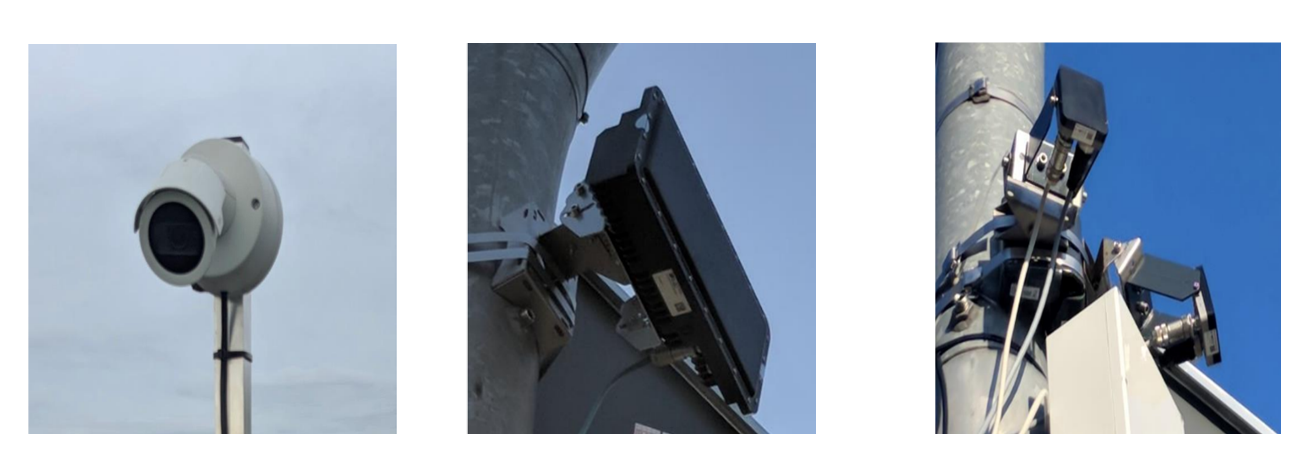
\includegraphics[width=0.9\textwidth]{paper-template/figs/Hardware.png}
        \caption{Camera, InnosenT Radar, RF Beam Radar}
        \label{fig:my_label}
\end{figure} 
Cameras are used to obtain high-resolution information, including vehicle position, waiting time, and class, which includes car, truck, bus, and bike.
InnoSenT radars, which can detect objects up to 350 m away and track them at 230 km/hr, are used.\\
There is one InnoSen radar sensor that measures 117 m to the east and 87 m to the north. In the motion zone, the radar provides the exact speed, class, and direction of the vehicle. Each time a new car enters the zone, the data is updated. In the presence zone, the radar measures the queue length and number of vehicles. The power supply is 24 Volts Direct Current (VDC), which is approximately 36 watts. The field of view for the radar is azimuth: 110°, elevation: 30°. [\citet{KI4LSA_presentation}]
There are two RF beam radar sensors that measure 70 m to 80 m and the object speed at 100km/h. The radar sends raw data to the edge computer, which runs Nvidia's Jetson-AGX-Xavier HW. Every second, raw data containing position, speed, and direction is sent. The field of view for the radar is azimuth: 110°, elevation: 30°. The RF beam radar is powered by approximately 3.6 watts. The radar is tested for 4 weeks in the first period and 2 weeks in the second period. [\citet{KI4LSA_presentation}]
Computer vision is used to interpret images from the video stream. The Yolo object detection is used to detect vehicles and classify them into four categories. 
\begin{figure}[h]
        \centering
        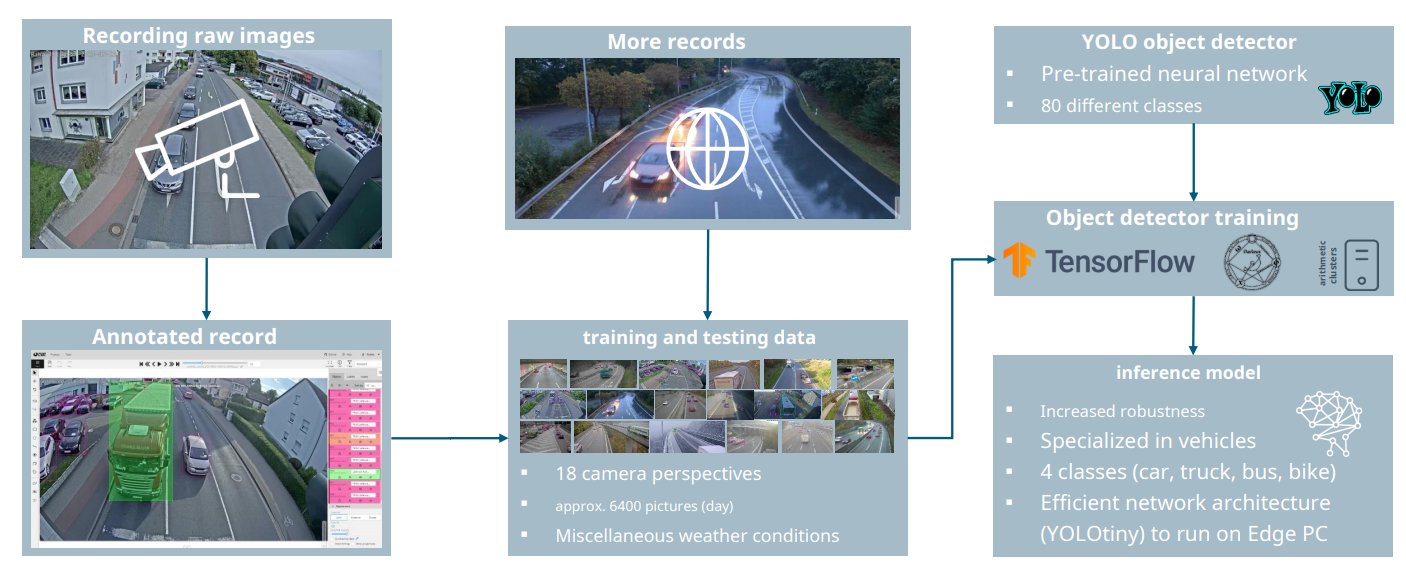
\includegraphics[width=0.9\textwidth]{paper-template/figs/computer vison.png}
        \caption{Computer vison pipeline}
        \label{fig:my_label}
\end{figure} 
The track and position accuracy metrics are obtained from the video stream for individual vehicles then a summary of metrics per lane is provided, including queue length and maximum waiting time. The methodology used to validate the computer vison is to compare the manuals of vehicles in both lanes to the machine-generated data. The result is 83\% accuracy across tracks.
   \subsubsection{Version of software used (Annex IV 1. c)}
The simulation model called LemgoRL is an open-source tool used to train and evaluate the Reinforcement learning agent.[\citet{traffic_signal_control_with_rl}] The model contains the realistic simulation environment "OWL322" intersection in Lemgo, a medium-sized town in Germany. It is built using SUMO, an open-source tool used to provide the required simulation environment. The environment for the 
simulation model is developed with python.[\citet{traffic_signal_control_with_rl}]
  \subsubsection{How the System is put to service (Annex IV 1. d)}
The AI system is put into service as the optimum solution to manage the traffic flow in the congested intersection which the current system is inadequate to handle. The system is also managed to be efficient between 10 to 15\% which is an economic gain as well as an environmental gain. The safety layer to double-check the results from the AI system ensure the safety by design principle deployed in the KI4LSA. 
  \subsubsection{Hardware the System is Running (Annex IV 1. e)}
\begin{figure}[h]
        \centering
        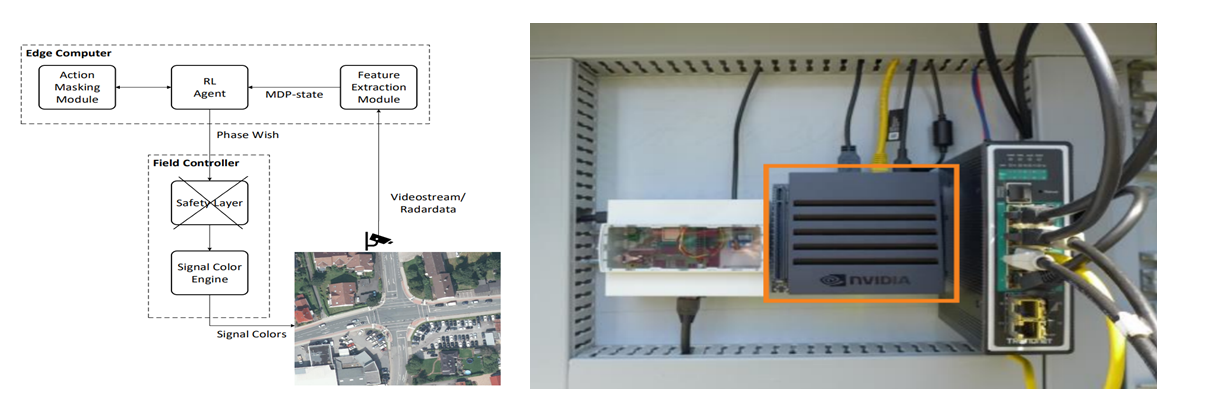
\includegraphics[width=0.9\textwidth]{paper-template/figs/edge computer.png}
        \caption{AI Hardware}
        \label{fig:my_label}
        \end{figure} 
The calculation runs on an edge computer at the control box of the real intersection. The AI system is powered by Nvidia Jetson AGX Xavier, with leading performance and power efficiency designed for the convergence of computer vision and AI. It is by far the most potent GPU-powered machine created for edge AI. It is also made to be energy-efficient. Equipped with a 7-way VLIW vision processor, 512-core Volta GPU with tensor cores, eight ARMv8.2 "Carmel" CPU cores, 16GB of LPDDR4x memory, 32GB of eMMC5.1 storage, two NVDLA deep learning accelerators, and 20x the performance and 10x the power efficiency of the Jetson TX2. [\citet{NVIDIA_Jetson_AGX_2022}] 
Evaluation and aggregation of the sensor data on a compact computer on site for determining vehicle position, speed, and class data processing. Data from camera or radar sensors are processed in real-time by a feature extraction module that transforms them into an state for the Reinforcement learning agent. [\citet{(Muller_et}] Based on that state, the RL agent selects the next phase in the traffic controller.

  \subsubsection{Where the AI System is a component of other products (Annex IV 1. f)}
  Does not apply to us.
  \subsubsection{Instructions of use for the user and installation instructions (Annex IV 1. g)}
  \begin{figure}[h]
        \centering
        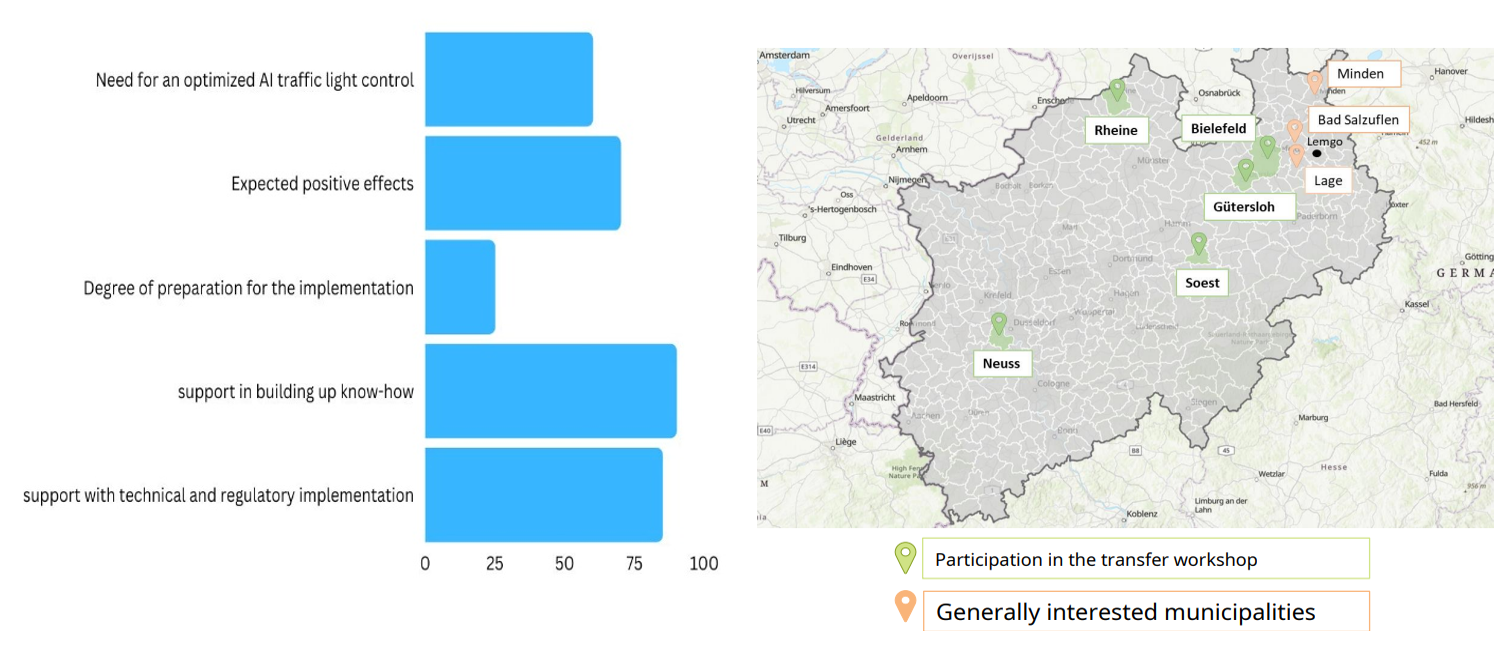
\includegraphics[width=0.9\textwidth]{paper-template/figs/Survey from the users.png}
        \caption{Survey from the 5 municipalities participated}
        \label{fig:my_label}
        \end{figure}
There is complexity in the system, and collaboration between regulatory bodies and research teams is more important than ever. This is achieved through multi-stakeholder workshops to achieve bench-marking solutions and project handover, and it has happened in the past.
Municipalities are among the stakeholders interested in implementing smart solutions for congested intersections.[\citet{KI4LSA_presentation}] The knowledge sharing is organized through workshops with the municipalities. The session covered results and findings from the discussion, technical requirements, and checking the status in relation to regulatory requirements for implementation. The evaluation from the workshop showed that the project can be implemented immediately  with  effort. The technical requirement includes auditing the existing infrastructure for implementing the system. The project handover happens in a phase as it involves know-how, and making AI familiarized to the municipal authority needs adequate time. After these steps, involving the public in understanding the safety of the system is crucial for the goal of the project.
  \subsection{Detailed description of AI System elements (Annex IV 2.)}
  Current traffic light controls are rule-based, the rigid rules do not apply to all traffic situations. In addition, the existing sensors – induction loops embedded in the asphalt – only roughly depict the traffic situation. \\
  Instead of conventional sensors, in the "KI4LSA" and "KI4PED" projects, researchers at the Fraunhofer Institute for Optronics, System Technologies and Image Exploitation IOSB, branch for industrial automation INA in Lemgo implement high-resolution camera and radar sensors that record traffic events more precisely. The number of vehicles waiting at the intersection can be recorded in real time, true to the lane. The average speed of the cars and the waiting time are also detected. The real-time sensors are combined with artificial intelligence, which replaces the rigid control rules.
  \subsubsection{Method and steps performed for development (Annex IV 2. a)}
  The AI for "KI4LSA" uses deep reinforcement learning algorithms. This machine learning method focuses on finding intelligent solutions to complex control problems. They built a realistic simulation model of the Lemgo junction where the tests took place and let the AI train countless iterations in this model. Beforehand, they transferred the measured traffic volume during rush hour to the simulation model so that the AI can work with real data. The result is an agent trained using Deep Reinforcement Learning, a neural network that represents the traffic light control.\\
  Deep reinforcement learning (deep RL) is a subfield of machine learning that combines reinforcement learning (RL) and deep learning. RL considers the problem of a computational agent learning to make decisions by trial and error. Deep RL incorporates deep learning into the solution, allowing agents to make decisions from unstructured input data without manual engineering of the state space. Deep RL algorithms can take in very large inputs (e.g., every pixel rendered to the screen in a video game) and decide what actions to perform to optimize an objective (e.g., maximizing the game score).
  \begin{figure}[h]
        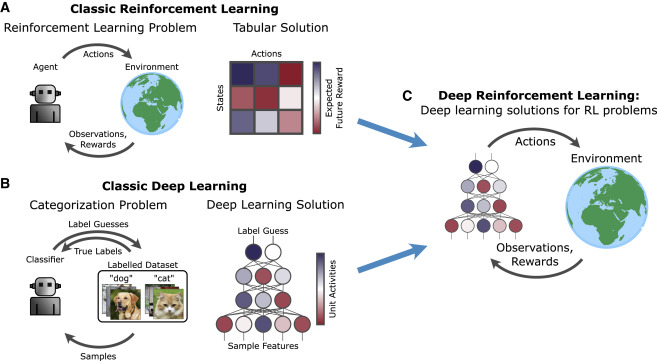
\includegraphics[width=0.9\textwidth]{paper-template/figs/DeepRL1.jpg}
        \caption{Deep Reinforcement Learning}
        \label{fig:my_label}
        \end{figure}
  \subsubsection{Design specifications of the system (Annex IV 2. b)}
  The system consists of additional sensors and edge computer at the traffic lights in order collect real time traffic data which is processed by the edge computer to make correct actions. The system also includes connection to services (e.g., Dashboard) and an interface between control unit and edge computer. To connect the edge computers to a central computer, they use standardized protocol Open Communication Interfaces for Road Traffic Control Systems (OCIT). To integrate AI in real operation, data exchange takes place using Ethernet. This allows for faster data exchange, scalability and reduce errors.
  
  \subsubsection{Description of the System architecture (Annex IV 2. c)}
  Agents in Deep RL algorithm typically uses neural networks to classify the input data into categories. The goal of the agent is to make decision based on collecting as much rewards as possible (cumulative reward). \\
Thus, the agent tries to minimise the travel time for vehicles and pedestrians. Learning and training involves adjusting the weights of neural network so that good actions are chosen to collect as much cumulative reward as possible.\\
 \begin{figure}[h]
        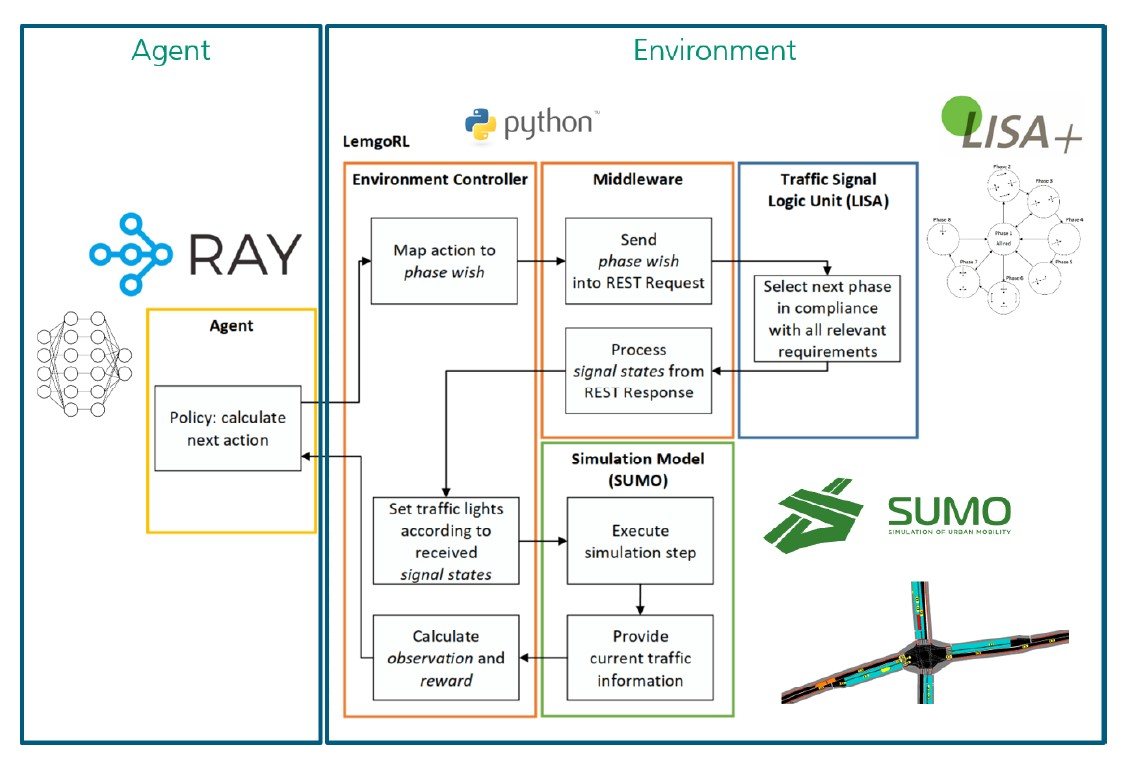
\includegraphics[width=0.9\textwidth]{paper-template/figs/sytemarchitecture.jpg}
        \caption{AI System Architecture}
        \label{fig:my_label}
        \end{figure} \newline
\textbf {Integration of AI in Real Operation:}\newline
The second part of the Deep RL system is the environment which provides the state and reward data back to the agent. The environment of KI4LSA is divided into 3 parts[\citet{KI4LSA_presentation}]:
\begin{enumerate}
\item 	LemgoRL : This unit maps the action to phase wish. It sends the phase wish into REST request so that valid states are chosen. According to the received signal states, LemgoRL sets the traffic lights into new state. It calculates the observations and rewards and allows the AI system to make a right decision.
\item Traffic Signal Logic Unit (LISA) : This unit makes sure the next phase/state chosen is in compliance with all relevant requirements. This ensures that any unknown state or wrong phase is not chosen.
\item Simulation Model (SUMO): SUMO is Simulation of Urban Mobility. Basically, this unit runs a simulation of the state and provide current traffic information for the LemgoRL unit to calculate rewards.
\end{enumerate}
 

  \subsubsection{Training data (Annex IV 2. d)}
  To ensure a fair comparison, they train each RL agent for each controller 5 times with different random seeds while they use the same set of random seeds for each controller. This makes in total
15 agents. The training is done in the LemgoRL framework.[\citet{KI4LSA_presentation}] They
calculate the average over all lanes respectively pedestrian
crosswalks and all 10 runs for the following traffic metrics:
\begin{enumerate}
\item queue: The length of the queue of waiting vehicles
(velocity < 0.1m/s) in a lane
\item wait veh: The maximum time a vehicle waits in a
lane when the signal color is red
\item speed: The average speed of all vehicles in a lane
\item wait ped: The maximum time a pedestrian waits for
a green signal at a crosswalk
\item stops: The avg. number of stops of a vehicle while
it approaches the intersection
\item travel time: The avg. time for a vehicle to cross
the intersection
\end{enumerate}
Also, they compute the cumulative reward a controller
collects during a run. For the reward function, we extend the
definition in [5] to include stops total, the number of
all vehicles stops in a lane at a given time t: \newline \newline
\begin{math}
r_{t+1} = -\sum_l (\alpha_q . queue_{t+1}[l]+\alpha_{w,veh}.waitveh_{t+1}[l] + \alpha_{w,ped}.waitped_{t+1}[l] + \alpha_{st}.stopstotal_{t+1}[l]) \end{math} \newline \newline
where l denotes an incoming lane or pedestrian crosswalk
of the intersection and \begin{math} \alpha_{q}, \alpha_{w,veh}, \alpha_{w,ped}, \alpha_{st} \end{math} are coefficients for weighting the individual components.\\
For all RL agents they used the Proximal Policy Optimization algorithm with the hyperparameters.\\
RL is data inefficient. Hence many training runs are necessary to optimize the algorithm and set the right hyperparameters. This is computationally intensive. Hence there is a need for parallelization of training process and use of high-performance hardware.\\
\begin{figure}[h]
        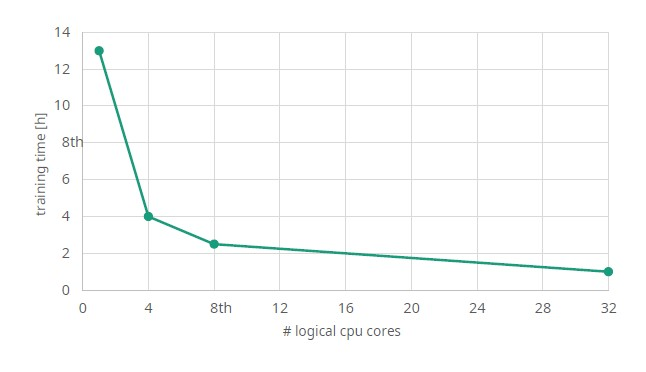
\includegraphics[width=0.9\textwidth]{paper-template/figs/trainingdata.jpg}
        \caption{Comparison of hardware requirement for training}
        \label{fig:my_label}
        \end{figure} \newline
Another concern is the simulation to reality gap. To reduce it and get results as close to real situation, noised data is introduced. Traffic volume, vehicle length, driving behaviour, weather, noise due to sensor, etc.  are just a few types. 
  \subsubsection{Human oversight needed (Annex IV 2. e)}
  Since Deep RL is used in the AI system, the results are obtained automatically. Basically the deep learning module is a black box and hence there is very less control over the methodology in which the result is obtained. To overcome this, there is a security layer which ensures that only results compliant with the traffic rules are considered. Human oversight can only be done in the form of type of deep learning model chosen and hardware used for the system. During simulation, results obtained are good but the same cannot be said when AI system is implemented in real scenarios. Rigorous testing needs to be done in order to use it for real scenarios.
  \subsubsection{Future changes to comply with High Risk System requirements (Annex IV 2. f)}
  To use the traffic light systems for pedestrians, Fraunhofer is working on the project KI4PED. Particularly vulnerable people such as the elderly or people with disabilities should benefit from this. The aim is to shorten waiting times and increase safety at traffic lights by longer crossing times. According to current studies, the green phases are too short for these groups of people.\\
  The buttons currently installed, mostly small yellow boxes, provide neither information about the number nor the age or even the infirmity of the passers-by. By implementing AI in combination with high-resolution LiDAR sensors, the project partners want to automate the process and automatically adjust and grade the crossing times to the needs of the respective pedestrians. Person detection and tracking is achieved based on LiDAR data using AI and implemented in an embedded system in real time.\\
  For reasons of data protection, we use LiDAR sensors instead of camera-based systems, since they represent pedestrians as 3D point clouds, and they cannot therefore be identified. LiDAR (Light Detection and Ranging) sensors emit laser beams to measure distances and detect the backscattered light. The distance to the object, i.e., to the person, is determined from the transit time of the light. These sensors are also robust against lighting, reflection, and weather influences. Their optimal positioning and orientation at the traffic light crossing will be examined as part of a feasibility study
  \subsubsection{Validation and Testing procedures (Annex IV 2. g)}
  In the validation, the accuracy was considered on the level of single image the AI gets its metrics 1 time per second based on 5 aggregated images, thus increasing robustness. Further increase in robustness can be achieved through using filters like compensating for large, obscuring vehicles. AI can be supplied with data using video cameras and image processing. \\
  Accuracy was used as a performance measure. The computer vision provided the accuracy of 83\% across all tracks. The results from the agent cannot be controlled as the Deep RL uses deep learning techniques; it basically is a black box. This is the reason a security layer is used to ensure that the results are in compliance with the traffic system.
  \subsection{Predicted and known limitations (Annex IV 3.)}
  
There are a few points where the robustness and accuracy of the system could be compromised.\\
At a very basic hardware level, the connection between the different traffic lights to the edge computer could be interrupted. The connection is done with 5 GHz WiFi which is not always perfectly stable. If it were interrupted and no data was sent from one of the cameras or radar systems, the timestamps would be wrong and the system would switch back to the conventional method of switching traffic lights.

The same mechanism is used when one of the sensors is not working properly and transmitting no data, the AI system would shut itself off and try to restart all the systems. If it were the other way around and the AI system died, the control device in the traffic light system would not receive data anymore and switch to the conventional traffic light system as well. [\citet{KI4LSA_presentation}]\\
At the software level, the first algorithm that could be wrong would be the YOLO (You only look once) neural net labeling the cars driving through the intersection and counting them. The accuracy of the computer vision across all lanes is about 83\% [\citet{KI4LSA_presentation}] which sounds like it is not enough but as it is only used for counting the cars and poses no risk to the security of the system as I will later show it doesn't matter much.\\
The KI4LSA system does not identify persons, as it is only used on cars so there's no risk of discrimination for different groups of persons based on details about the persona.

It could be possible that one car would be determined as not important enough to let through because of a lot of cars in other lanes, this poses a psychological harm to some drivers and potentially a problem to the safety of the junction but this is managed by the risk management system.

Possible risks include wrong traffic lights determined by the system based on any amount of errors mentioned before or unforeseen errors.
If there are faults in the commands by the system it would very likely lead to crashes at the junction which could include human harm and even death. As there are also pedestrians walking around it could also involve them as innocent bystanders. This makes it clear again why this should be considered a high-risk system and also why we made the environment and variables of the system "safe-by-design" which I will elaborate on later.

As this was a research project the system and findings were measured and overseen by many people. This was made possible by different dashboards measuring the different data collected from the traffic lights as well as data collected by the computer vision system.
\begin{figure}[h]
        \centering
        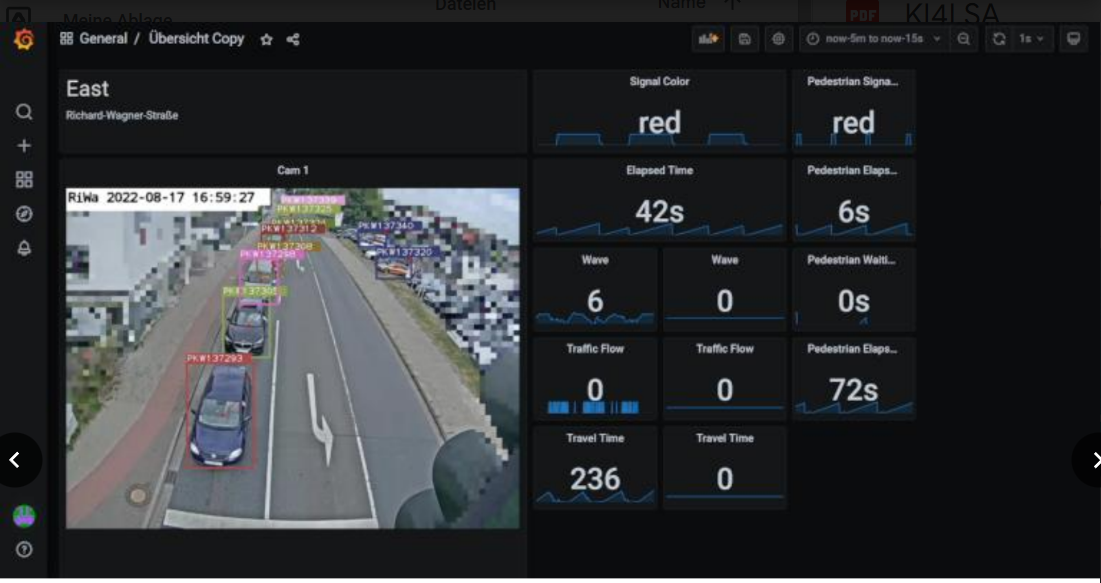
\includegraphics[width=0.8\textwidth]{paper-template/figs/dashboard.png}
        \caption{Camera view of the junction and different data}
        \label{fig:my_label}
\end{figure}

As seen below, it is also possible to view and compare the waiting times and get a general overview of the traffic pass-through. Which is important for monitoring the performance of the system when deployed.\\

\begin{figure}[h]
        \centering
        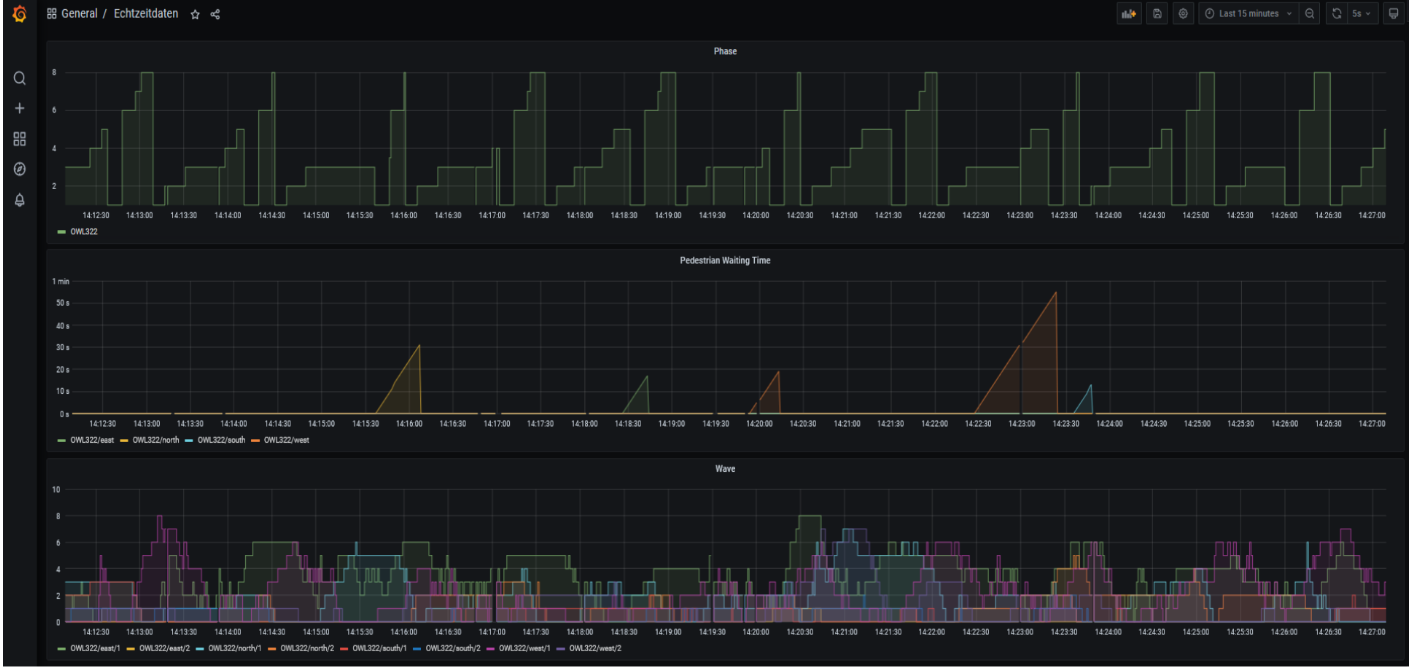
\includegraphics[width=0.9\textwidth]{paper-template/figs/dashboard_time.PNG}
        \caption{Comparison and overview of the different wait times and flows.}
        \label{fig:my_label}
\end{figure}

Although it seems simple trying to understand the system's decisions is often very complex and is not really feasible in practice. This is why the environment and algorithm were made "safe by design" to not have to worry of any possible risks about the system going rogue. \newline

  \subsection{Risk management system (Annex IV 4.)}
Because the AI system developed is used in infrastructure it is determined as a "High-risk" AI system and therefore needs according to Article 9 of the AIA [\citet{ai_act}] a Risk management system.

Because the system should be inherently safe it was decided to do a "safe-by-design" approach towards the project with an extra security layer.
In the beginning, it was determined too risky for the system choose each light independently without some inherent constraints. That's why there was a phase system introduced to LemgoRL.

\begin{figure}[h]
        \centering
        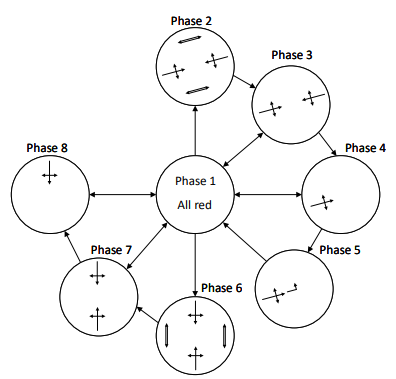
\includegraphics[width=0.8\textwidth]{paper-template/figs/risk_management_2.png}
        \caption{Traffic phases of LemgoRL and their transitions presented as a graph. The single-lined arrows represent the permitted directions of travel for vehicles and the double-lined arrows indicate that pedestrians are allowed to cross the street in the respective direction.}
        \label{fig:my_label}
    \end{figure}
The AI can only choose between the eight different action spaces (1-8/0-7 in computer science). This makes sure that there are no contradicting lights so for instance, a phase transition from phase 2 (vehicles west and east as well as pedestrians north and south) to phase 3 (only vehicles west and east) requires phase 2 to be active for at least 10s, so that pedestrians can safely cross the street before they get a red signal. This ensures that there is no way the system could make a contradicting choice. [\citet{traffic_signal_control_with_rl}]

With those constraints it would still be possible for the AI to for example make a 3 $\rightarrow$ 1 $\rightarrow$ 3 sequence if there are a lot of vehicles east and west. This would pose a bad psychological effect on individual drivers as it is from their view not at all logical. To counteract this a psychological action mask (A common mechanism used in reinforcement learning) is used which basically means that the model "knows" unwanted behaviour and is prohibited from doing so.

This was also tested with and without the psychological mask and although traffic flow is better without the mask it was determined that this poses a risk to road safety.

To fulfill the requirements set out in Article 9 paragraph 2 of the AIA [\citet{ai_act}] there is also an iterative process running in the system checking that the aforementioned requirements are always kept. There is also a mechanism in progress checking that the model still produces the wanted results and that there are no accidents due to the new system.

To double-check the safety constraints are upheld, the phase system is also placed as a safety layer in an independent system between the AI model and the traffic light controllers. So basically the Reinforcement agent only gives recommendations that the Safety Layer has to approve before the controller acts on them.

\begin{figure}[h]
        \centering
        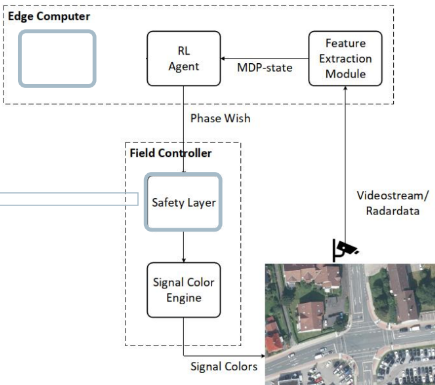
\includegraphics[width=0.8\textwidth]{paper-template/figs/risk_management_1.PNG}
        \caption{Safety layer placed in the traffic light system.}
        \label{fig:my_label}
    \end{figure}
    
The measures were tested beforehand in the simulation and showed great results. It was also tested in reality at the beginning of 2022 during which time no accidents occurred. The AI system makes perfectly safe recommendations in 1 out of 10.000 scenarios and when it doesn't the safety layer is there to protect the integrity of the junction.

The system poses a particular risk to children because they are passengers of the cars crossing the street but as no children are identified or are a variable in our model we did not that them into particular consideration.


\subsection{EU declaration of conformity (Annex IV 7.)}
This is the EU Declaration of Conformity for the AI System by Fraunhofer. I have to declare that this was drawn up by Benedikt Schwankner who is in no way associated with Fraunhofer and does not have all of the information about the development process. This document holds no legal value.
\begin{enumerate}
    \item The unique identification of the System is "KI4LSA" by Fraunhofer IOSB-INA
    \item Provided by Fraunhofer IOSB-Ina in Campusallee 1, 32657 Lemgo, Germany
    \item This declaration of conformity is issued under the sole responsibility of Fraunhofer IOSB-INA
    \item The AI system is in conformity with the AIA and especially the requirements for High-Risk Systems
    \item No harmonised standards of the EU were used but state of the art frameworks and tools by other providers recognized and reviewed by peers
    \item The system was presented to the BMDV (Bundesministerium für Digitales und Verkehr) and BMWK (Bundesministerium für Wirtschafts und Klimaschutz) was notified as a NANDO authorised body
    \item Drawn up in Munich on 02-12-2022 by Benedikt Schwankner as a dummy with no function at Fraunhofer
\end{enumerate}


\subsection{Evaluation in post-market phase (Annex IV 8.)}
  
  A post-market monitoring and a risk management system will be established according to Art. 61 of the AI Act proposal [\citet{ai_act}].
Monthly evaluations will be conducted by the provider to ensure the AI system performance. Required data will be gathered through automatic recording (logs) locally and give therefore the possibility to trace events. The following date will be recorded: start date and time and end date and time of each use, the reference database and the input data (Art. 12). 

Furthermore, said evaluations will be published for reasons of transparency (Art.13) and include: the identity and the contact details of the provider, the characteristics, capabilities and limitations of performance of the AI traffic light system, all changes made, expected lifetime of the AI system and human oversight measures.
The data can also be accessed through the provided dashboard [\citet{KI4LSA_presentation}], as required in Art. 14 and performed by employees of the municipality. Employees are given necessary instructions and training to perform the required tasks. The dashboard also gives the possibility to intervene in an AI related operation and bring it to a halt.

Should technical changes occur, will the technical documentation  be updated accordingly (Art.11) To meet the requirements in Art. 15 the connection between the traffic lights and the employees is high-level encrypted and state of the art cybersecurity is in place. There is always a fallback option in case errors occur [\citet{seick}].

  \section{Discussion And Ethical Analysis}
  \\
  
  When analysing ethical aspects in regards of the AI Act, one has to take into consideration that the development of the proposal itself has its origin in the High-Level Expert Group on AI [\citet{HLEG_2019}], which already set up ethics guidelines for trustworthy AI in 2019 [\citet{ai_act}]. Therefore it can be said that the importance of ethical evaluation of AI was thought as an important part of the act from the beginning. \\
  
As AI systems should improve individual and collective wellbeing, the Ethics Guidelines of the HLEG propose four ethical principles [\citet{HLEG_2019}]: respect for human autonomy, fairness, explainability and prevention of harm. In the following section these ethical imperatives will be discussed on the example of KI4LSA of Fraunhofer IOSB-INA. The project itself is only deployed in real world usage applying a second security layer as described in the introduction. For the analysis though it is assumed that the AI is working without these restrictions while taking them in consideration if necessary.

The first ethical principle: respect for human autonomy is requiring the AI system to use a human-centric design and not unjustifiably subordinate, coerce, deceive, manipulate, condition or herd humans (ibid.). In this case of traffic lights, the already used system is human-centric as being focused on organising human travel. The AI is merely improving this system, aiming for a reduction of travel time. KI4LSA showed an improved traffic flow of 10\%
and effects on traffic in the surrounding area [\citet{KI4LSA_presentation}].  It is in its core expanding human autonomy and therefore in line with this ethical principle.

The principle of fairness covers many different interpretations of fairness, be it on the level of the individual, like discrimination, or societal fairness, like equal opportunities. As traffic lights are a public good, everybody has access and the used sensors do only recognize vehicles, without differentiation. A whole different case is the sister project KI4PED, which aims to improve traffic lights for pedestrians and does not analyse cars, but humans - especially with regards to their disabilities, which leads to longer green phases. This is highly personal data and would raise a lot of other questions. But this is not the case for KI4LSA and as a consequence it is a fair AI system.

With being a fair system, comes the requirement of identifiable and explicable decision making. While in other cases explicability of AI is of very high relevance (i.e. judicial decisions), one can argue that this is not the case here. Humans are accustomed to the behaviour of traffic lights and even though on an individual level one could feel unsure about the effectiveness of red and green times, this is highly subjective and already the case without an AI system in place. Again in KI4PED, the differentiation between disabilities and the decision making would have to be much more explicable. As cars are all considered equal (despite given differences in size and acceleration), there is no need for further explanation.

Lastly it can be argued that the prevention of harm is the most important principle in this list. It does not only cover mental and physical integrity, but also human dignity and the natural environment. Handing over traffic regulation to an AI might pose the risk of accidents resulting from miscalculations and high speeds. Humans trust traffic lights to show correct signals and behave accordingly.

First of all one could raise questions on the sensors, which analyse incoming traffic. Bad weather conditions like rain, fog or snow can challenge the system, the experiment showed. Anyhow video and radar sensors deliver an accuracy of 83\% 
(ibid.), much higher than regular sensors and can also provide data at night time. If problems occur, the AI would restart itself and the second security layer would take over. While sensor data is an important start, the real question lies in the decision making of the system. To make the AI as secure as possible, Reinforced Learning was applied. This training process is pushing the AI towards improving the traffic flow and avoiding mistakes. It was counted as a mistake when the AI was making decisions which contradicted the requirements of the second security layer, e.g. red and green signals on opposing sites. As a consequence the AI is trained within the boundaries of the security layer while improving the traffic flow. As said in the beginning, the real world usage is still using a real second security layer in addition to the trained security layer.

An interesting side effect can be seen when taking the harm of the natural environment into the focus. The study (ibid.) showed a reduction of 10-20\%
 of CO2 emissions while applying the system in contrast to standard regulation. One could argue the AI is not even not harming the environment, but improving it instead.
Taking these points into consideration one can argue that the KI4LSA traffic light system is preventing harm as required in the guidelines.\\

Usually tensions occur between the principles described above. In the case of improved traffic lights like KI4LSA though, the values align: more human autonomy is given through improved traffic flow, fairness and explainability are given in anonymised traffic and prevention of harm is assured through various security layers, while less greenhouse gas emissions occur. This can all be explained by the fact that this AI application is merely improving an already existing, understood and accepted concept of human-machine behaviour i.e. traffic regulation, which reduced the number of issues, compared to other AI applications.\\

\\

Analysing the KI4LSA system from an external perspective one can raise multiple further, more fundamental points as ethical questions can go deeper than recommended by the guidelines of the High-Level Expert Group on AI.

First issue that comes to mind is the exclusive focus on automotives. The current approach is solely relying on scanned vehicles like cars, lorries and buses. It is not optimised for motorcycles and bikes, which can be seen as an unfair towards humans preferring to ride those for various (especially economical) reasons. Car drivers might profit from a better traffic flow, but this could also lead to higher speeds, more noise pollution and higher risk for other road users, especially pedestrians. Other traffic participants might not as much profit from the AI application which might disadvantage them compared to car drivers directly and indirectly. Not being able to be part of the car traffic, might motivate people to switch to cars instead, which could zero out the effect because of more cars on the road. 

In an even bigger context, encouraging people to use individual mobility instead of public transport could slow down traffic in the long run. Improving car traffic without similar or greater improvements in public transport could nullify the positive effects in the future.

Connected with all these arguments is the issue of climate change: giving incentives to stick with a certain traffic system that is responsible for 19\%
of Germany's greenhouse gas emissions [\citet{umweltbundesamt}], by improving it might not be the way to fight the climate crisis effectively. Of course the improved traffic flow can locally reduce emissions, as said before, but the overall concept of individual mobility should be considered problematic, looking at the far to low emission reductions in the mobility sector (ibid.). \\

Applying the ethical imperatives from before, fairness towards people without a car is questionable and fairness towards future generations might also be when emissions are not reduced sufficiently. This goes hand in hand with harm to current and future populations and therefore contradicts the points made before on a bigger scale.

On the other hand development in AI usage in traffic could also be a first step towards a new way of traffic with autonomous vehicles and vehicle-to-x communication. One could argue that in the upcoming future cars could be first of all fully electric, which, provided coming from a renewable power source, would not be harmful to climate and the environment. And with a Sharing Economy the number of vehicles on the street (driving and standing) could be reduced massively. This in combination with said traffic light system, could lead to a very efficient traffic flow without the downsides mentioned above.\\

The KI4LSA AI traffic light system meets all ethics requirements of the HLEG guidelines and can therefore be applied in the EU. To what extend one wants to put the consequences of further improved individual mobility into considerations, is something for society to debate and decide on. 



  \addcontentsline{toc}{section}{References}
 \bibliographystyle{apalike} 
\bibliography{bib}
\end{document}
